\documentclass[a4paper,12pt]{scrartcl}
\usepackage[margin=2cm,bindingoffset=0cm]{geometry}
\usepackage{ucs}
\usepackage[utf8x]{inputenc}
\usepackage[ngerman]{babel}
\usepackage{fontenc}
%\usepackage[pdftex]{graphicx}
\usepackage{listings}
\usepackage{amssymb}
\usepackage{amsmath}
\usepackage{wasysym}
\usepackage{graphicx}
\usepackage[pdftex]{hyperref}
\author{
Verena Käfer (2551188),\\
Niklas Schnelle (2573250),\\
Peter Vollmer (2553704)}
\date{erstellt am 08.12.2010\\
Version: 1.2}
\title{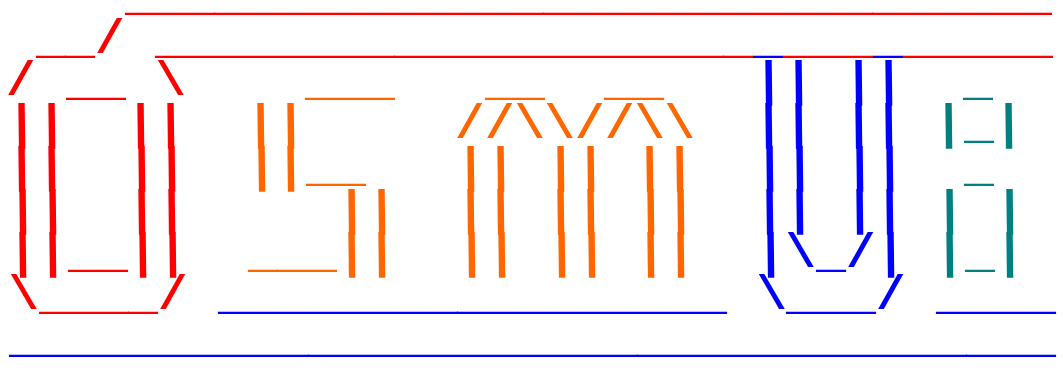
\includegraphics[width=15cm]{../projektplan/Logo_Osmui.png} \\ 
Entwurf von OsmUi}

\begin{document}
\maketitle
\newpage
\tableofcontents
\newpage

\section{Einleitung}
Die folgenden Abschnitte beschreiben den Entwurf und die Architektur von OsmUi.
\subsection{Das Software-System}
OsmUi stellt eine Benutzeroberfläche für das Kommandozeilen-Tool Osmosis dar. Die Implementierung erfolgt in Java 6, die Oberfläche wird mit Swing realisiert. Für die graphische Darstellung der Pipelines wird auf JGraph zurückgegeriffen. Die Pipelines werden entweder in smu-Dateien gespeichert oder als Kommandozeilenscripst exportiert.
\subsection{Entwurfsprinzipien}

\subsection{Überblick über den Entwurf}
In den folgenden Abschnitten werden zuerst die Architektur (Kapitel 2) und dann die einzelnen Komponenten (Kapitel 3) beschrieben. Die genaue Dokumentation der Klassen und Methoden erfolgt direkt im Programm als JavaDoc. Desweiteren soll dieses Dokument, die Entwurfsentscheidungen dokumentieren.

\section{Architektur}
Osmui setzt sich aus mehreren Komponenten zusammen. Diese sollen so organisiert werden, dass der Zusammenhalt innerhalb der Komponenten groß und die Kopplung zwischen ihnen möglichst klein ist. Zur Strukturierung des Systems sollen weiterhin GUI-Komponenten klar von den dahinter liegenden Modellen getrennt werden. Da OsmUi jedoch selbst Oberfläche für ein Kommandozeilenwerkzeug ist, existiert keine klare Frontend/Backend-Trennung.\\
Im folgenden sind die Komponenten beschrieben, wobei jeder Komponente im später System einer Java-Klasse entspricht.

%\subsection{Komponentenübergreifende Funktionen}

\section{Komponenten}
\subsection{Komponente: TaskBox}
Die TaskBox implementiert eine GUI Komponente die alle zum momentan selektierten Task kompatiblen Tasks anzeigt. Ist kein Task selektiert zeigt sie nur die Tasks an, die keine Vorbedingungen haben. Auch kann über sie ein Task zum TaskModel hinzugefügt werden.
\subsubsection{Schnittstelle}
Die TaskBox implementiert die Interfaces TaskSelectEventListener und TaskForAddEventListener. Der  Konstruktor übernimmt ein PipeModel, in das die TaskBox neue Tasks einfügen soll. 
\begin{center}
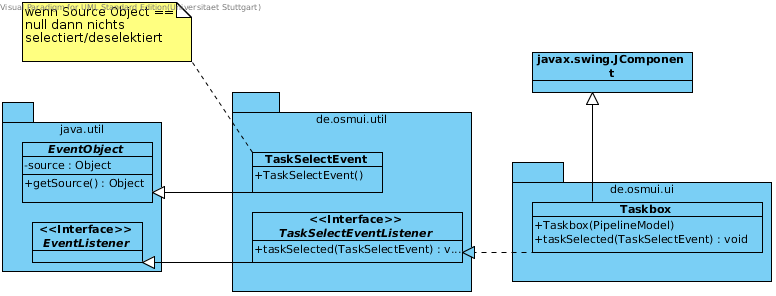
\includegraphics[width=17cm]{Schnittstelle_TaskBox.png}
\end{center}
\subsubsection{Protokoll}
Nach der Konstruktion muss die TaskBox noch als EventListener registriert und zur Benutzeroberfläche hinzugefügt werden.
%\subsubsection{Verhalten}

%\subsubsection{Interne Realisierung}
\subsubsection{Realisierte Anforderungen}
Diese Komponente ermöglicht das Hinzufügen von neuen Tasks.

\subsection{Komponente: PipelineBox}
Die PipelineBox zeigt die aktuelle Pipeline an und ermöglicht dem Benutzer Tasks zu selektieren, zu verschieben und zu löschen. 
\subsubsection{Schnittstelle}

\subsubsection{Protokoll}
Wird ein Tasks selektiert, so wird ein TaskSelectEvent ausgelöst. Wird kein Task selektiert, so wird ein TaskSelectEvent mit Source gleich null ausgelöst. Ein Doppelklick auf ein Task löst ein TaskSelectEvent und ein TaskDoubleclickEvent aus.
\subsubsection{Verhalten}

\subsubsection{Interne Realisierung}
\subsubsection{Realisierte Anforderungen}

\subsection{Komponente: ParameterBox}
Die ParameterBox zeigt die Parameter des aktuell selektierten Tasks an und ermöglicht dem Benutzer diese zu ändern. 
\subsubsection{Schnittstelle}
\begin{center}
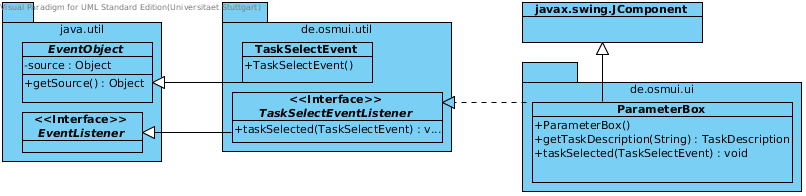
\includegraphics[width=17cm]{Schnittstelle_ParameterBox.png}
\end{center}
\subsubsection{Protokoll}
\subsubsection{Verhalten}
\subsubsection{Interne Realisierung}
\subsubsection{Realisierte Anforderungen}

\subsection{Komponente: Application}
Die Application stellt das Hauptfenster bereit, in dem alle Oberflächenelemente enthalten sind.
\subsubsection{Schnittstelle}
\subsubsection{Protokoll}
\subsubsection{Verhalten}
\subsubsection{Interne Realisierung}
\subsubsection{Realisierte Anforderungen}

\subsection{Komponente: TaskManager}
Der TaskManager verwaltet die Informationen zu Taskstypen , prüft Kompatibilitäten zwischen Tasks und dient als Factory für Tasks.
\subsubsection{Schnittstelle}
\begin{center}
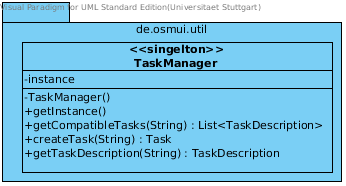
\includegraphics[width=8cm]{Schnittstelle_TaskManager.png}
\end{center}
\subsubsection{Protokoll}
\subsubsection{Verhalten}
\subsubsection{Interne Realisierung}
\subsubsection{Realisierte Anforderungen}

\newpage
\subsection{Komponente: PipelineModel}
Das PipelineModel hält die interne nichtgrafische Representation der Pipeline und bietet Schnittstellen für die Verwaltung von Tasks aus der Pipeline und der Validierung einer Pipeline. 
\subsubsection{Schnittstelle}
\begin{center}
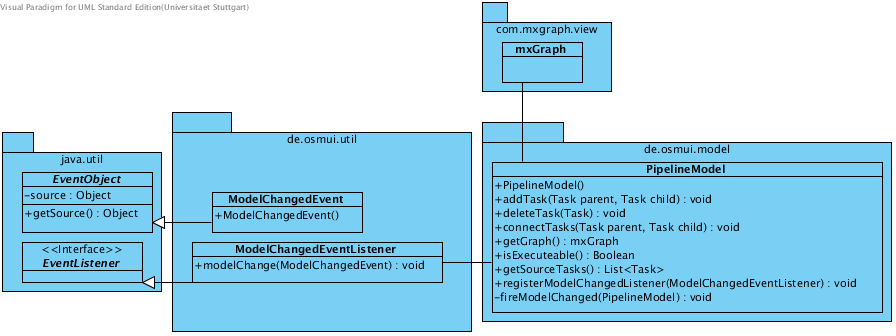
\includegraphics[width=17cm]{Schnittstelle_PipelineModel.png}
\end{center}
\subsubsection{Protokoll}
\subsubsection{Verhalten}
\subsubsection{Interne Realisierung}
\subsubsection{Realisierte Anforderungen}


\subsection{Komponente: PipeImEx}
Die Komponente PipeImEx übernimmt die Funktionalität des Importierens und Exportierens.
\subsubsection{Schnittstelle}
\begin{center}
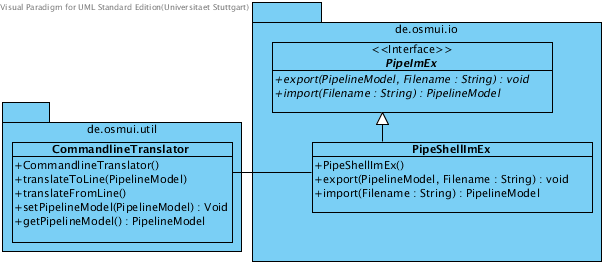
\includegraphics[width=17cm]{Schnittstelle_PipeImEx.png}
\end{center}
\subsubsection{Protokoll}
\subsubsection{Verhalten}
\subsubsection{Interne Realisierung}
\subsubsection{Realisierte Anforderungen}


\subsection{Komponente: Help}
Die Komponente Help übernimmt die Funktionalität der Hilfe.
\subsubsection{Schnittstelle}
\subsubsection{Protokoll}
\subsubsection{Verhalten}
\subsubsection{Interne Realisierung}
\subsubsection{Realisierte Anforderungen}

\subsection{Komponente: BoundingBoxChooser}
Die Komponente BoundingBoxChooser übernimmt die Funktionalität um einen Kartenausschnitt grafisch auszuwählen.
\subsubsection{Schnittstelle}
Die Schnittstellen übernehmen die API.
\subsubsection{Protokoll}
\subsubsection{Verhalten}
\subsubsection{Interne Realisierung}
\subsubsection{Realisierte Anforderungen}

\subsection{Komponente: I18N}
Die Komponente I18N übernimmt die Funktionalität der Internationalisierung.
\subsubsection{Schnittstelle}
\begin{center}
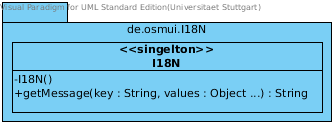
\includegraphics[width=8cm]{Schnittstelle_I18N.png}
\end{center}
\subsubsection{Protokoll}
\subsubsection{Verhalten}
\subsubsection{Interne Realisierung}
\subsubsection{Realisierte Anforderungen}

\subsection{Komponente: IPipeStore}
Die Komponente PipeStore übernimmt die Funktionalität des Ladens und Speicherns von Pipelines.
\subsubsection{Schnittstelle}
\begin{center}
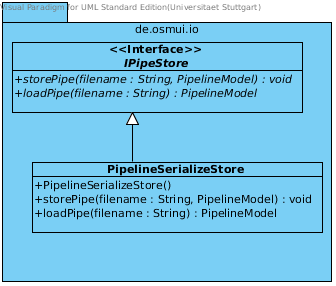
\includegraphics[width=8cm]{Schnittstelle_IPipeStore.png}
\end{center}
\subsubsection{Protokoll}
\subsubsection{Verhalten}
\subsubsection{Interne Realisierung}
\subsubsection{Realisierte Anforderungen}

\subsection{Komponente: ConfigurationsManager}
Die Komponente ConfigurationsManager übernimmt die Funktionalität der Konfiguration von OsmUi.
\subsubsection{Schnittstelle}
\begin{center}
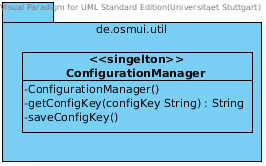
\includegraphics[width=7cm]{Schnittstelle_ConfigurationManager.png}
\end{center}
\subsubsection{Protokoll}
\subsubsection{Verhalten}
\subsubsection{Interne Realisierung}
\subsubsection{Realisierte Anforderungen}

\subsection{Verbindungen}

\section{Externe Schnittstellen}
\subsection{Dauerhafte Datenspeicherung}
Die geplante Implementierung, sieht vor Pipelines aus/in bash- und bat-Scripten zu importieren/exportieren, Pipelines aus der Zwischenablage zu importieren und aus/in .smu Dateien Piplines zu Laden/Speichern. Außerdem soll die Programmkonfiguration in in das Heimat-/Konfigurationsverzeichnisses des Benutzers gespeichert werden. Diese Speicherung erfolgt in einem für Menschen lesbaren XML Format in eine .conf Datei.
\subsubsection{Datei/Datenbank: .smu}
In dieser Datei wird die Pipline. Um die Daten in/aus dieser Datei zu speichern/laden wir das Serialisierungsverfahren von Java benutzt 
\subsubsection{Datei/Datenbank: .conf}
Diese  Dateiformat dient dazu die Systemeinstellungen von Osmui zu speichern die geschieht im XML-Format. Zu den zu speichernden Informationen gehören der Osmosis-Pfad.
\subsubsection{Datei/Datenbank: .dat}
Dieses Dateiformat dient dazu ein Script bereitzustellen, mit dem der Benutzer den generierten Osmosis Aufruf unter Windows Systemen leicht ausführen kann. Dies wird dadurch realisiert, dass der Osmosispfad mit den zugehörigen Tasks und deren Parametern der ersten Zeile steht.
\subsubsection{Datei/Datenbank: .sh}
Dieses Dateiformat dient dazu ein Script bereitzustellen, mit dem der Benutzer den generierten Osmosis Aufruf unter Unix Systemen leicht ausführen kann. Dies wird dadurch realisiert, dass als Header \glqq \#!/bin/sh" geschrieben ist. In der darauf folgenden Zeile befindet sich der Osmosis-Pfad mit den zugehörigen Tasks und deren Parametern.
%\subsection{Externer Zugriff}

%\subsubsection{Schnittstelle: XYZ}

\appendix%

\section{Anhang}

\section{Literatur zum Entwurf}
\subsection{Entwurf}
\subsection{Entwurfsmuster}
\section{Versionshistorie}
\begin{itemize}
\item Version 1.0 8.12.2010 : Initialisierung
\item Version 1.1 9.12.2010 : Komponentennamen festgelegt
\item Version 1.2 10.12.2010 : Klassendiagramme für Komponenten hinzugefügt
\item Version 1.3 11.12.2010 : Komponentenbeschreibungen, Externe Schnittstellen hinzugefügt
\end{itemize}

\end{document}